\documentclass[11pt,a4paper]{book}

\usepackage[utf8]{inputenc}

\usepackage{graphicx}

\usepackage[english]{babel}
\usepackage[T1]{fontenc}

\usepackage{amsmath}

\begin{document}

\title{Smart Mobility Lab \\
SML World 2.0 Reference and User Manual}

\maketitle

\tableofcontents

\part{Reference Manual}


\section{Referenced documents and websites}
\begin{tabular}{| l | l | p{80mm} |}
\hline
RD1. & SMLWorld.pdf & \textit{Documentation of previous version of the SML World} \\
\hline
RD2. & http://www.ros.org/ & \textit{Robot Operating System website} \\
\hline
\end{tabular}


\chapter{The SML World}
SML World refers to the demonstration environment of the Smart Mobility Lab. It contains all vehicle models, controls, graphics, traffic intelligence and coordination of the different subsystems used by any simulation. The system is based on the Robot Operating System (ROS) to enable execution of parallel processes. This version of the SML World builds on a version that did not utilize ROS, but has converted and further developed some of the previous vehicle models, road modules and visualization software, refer to RD1. for a closer description of their structure.

\chapter{System Setup}
\section{Hardware setup}
\subsection{The Qualisys positioning system}
The Smart Mobility Lab is equipped with the motion capture system \textit{Qualisys} that uses high speed infrared cameras. The cameras pick up any reflected infrared light and subsequently all lab windows should be covered to limit the amount of sunlight that comes in whenever the system is being used. There is a total of 12 cameras with some coverage overlap that are calibrated for the entire open space in the lab, which forms a (three dimensional) cube. The system requires occasional re-calibration to function well.

When the system is started the user is requested to select or create a project. A project stores and handles all 3D objects that have been defined for it. The project alias \textit{labhybrid2} currently contains definitions for the 1:32 trucks, 1:14 trucks, Iris quadrocopters and various obstacles that are most commonly used in the lab. Projects containing definitions of other lab equipment such as the Nexus robots can be found in the list. 

The system identifies each object based on a unique pattern of four reflectors attached to the object. New objects are then defined using the Capture tool in the Qualisys GUI.


\subsection{Projectors and screens}
There is a projector mounted in the ceiling meant for ground projections. Note that the remote used to switch it on uses infrared light and hence the Qualisys system cannot be active when starting the projector.

The lab is equipped with three ELO 32'' touch screens. Drivers for those screens are available for both Windows and Ubuntu systems on the ELO website. Note that the ELO drivers cannot handle multiple monitors so any additional screens connected to the same PC must be mirrored in order for the system to function. In a case where a GUI for the SML World is being controlled from the ELO touch screen, one must then run the SML World ROS application on both the ELO PC and another PC and define one as the master and the other as slave. Refer to the chapter ''Running ROS across multiple machines'' on the ROS wiki in RD2. Make sure that the firewall of both PCs allow traffic on the defined ip address. 

\subsection{Moving and stationary objects}
There are two types of scaled model Scania trucks available in the SML: three Tamiya 300056323 56323 1:14 Electric RC truck and nine Siku 1:32 RC trucks.

Various stationary objects used for previous SML demonstrations are also available in the lab.

\section{Software setup}
As mentioned above, the SML world is since early 2016 based on the Robot Operating System (ROS, please refer to RD2. for more information). As of now stabel versions of ROS is only available for Ubuntu. The python module \textit{mocap} has been developed to retrieve real time Qualisys data for the various SML applications using radio controlled trucks.

\chapter{Key SML World ROS Nodes}
As the SML World is a highly dynamic platform under constant change, this chapter will merely present the key nodes of the SML World ROS network rather than all that are available. The three nodes that make up the fundamental features of the SMl World are the road network, the visualization and the SML World central nodes. In addition this document also describes the nodes that make up the vehicle and certain other simulated objects.

\section{The SML World central}
SML World Central is the central node responsible for outputting the world state of the entire world. This includes the state of all vehicles, the current traffic status of the world, and the bussing system. All vehicles connect to this node, and it is the only node directly connected with the visualisation.

\section{The visualization}
\subsection{Pygame}
The visualization of the simulation relies entirely on the python game engine \textit{pygame}.

\section{The road network}
\label{sec:road}
The road network is defined by an XML file that describes segments referred to as \textit{lanelets}, which are made up of a various number of nodes. Each node corresponds to a coordinate pair which in turn describes one point on the road. Each set of nodes, or lanelet, is then related to other lanelets to form ways. Each network of ways must be given a reference point - an origin - which technically is a node that is decoupled from the rest of the network. The graphical tool Java Open Street Map (josm) is commonly used to draw the lanelets and determine their lanelets and possible tags. Refer to section 3 in RD1 for a closer description of open street map editing and the structure of the road network. \\

\noindent The node\_id is used by simulated vehicles to calculate trajectories. More precisely, vehicles use the given node ID:s to calculate the most efficient loop containing the given node ID using the Dijkstra algorithm to generate trajectories. The road network provides a service to allow vehicles to receive the surrounding area and will plot a trajectory through the road network to a given node. This is the higher level functionality that is separated completely from a low level controller.


\section{The vehicle and other simulated objects}
\label{sec:vehicles}
This section described the recent additions to the vehicles and other simulated objects in the SML World. To understand the basic vehicle structure refer to Section 2.1 in RD1. \\

\noindent Each vehicle runs on a ROS node. There are various subclasses vehicles, which define either the high level functionality—how the vehicle plans paths, reacts to traffic, and communicates with other vehicles—and low level functionalities, such as obtaining radar readings and turning. \\

\noindent The available vehicle classes in the SML World are the following:
\begin{itemize}
\item BaseVehicle: most basic form of vehicle, without any simulated sensors or extra featuers.
\item DummyVehicle: corresponds to the basic implementation of a smart vehicle.
\item Bus
\item TruckVehicle: used to virtually track the physical trucks
\item SmartWifi: vehicle class containing features for V2V functionality
\end{itemize}

\subsection{Vehicle to Vehicle Communication}
Vehicle to vehicle communication has been implemented for the SmartWifi class and aims at enabling a simulation of realistic information exchange between smart vehicles. Each smart vehicle is equipped with a radar that will trigger inter vehicle communication between any vehicles within the range of the radar. Note that the radar is enabled for both vehicle and pedestrian detection. Refer to Section 4.3.1 in RD1. for information about the sensor simulation and virtual radar implementation. \\

\noindent The V2V is used for the following:
\begin{itemize}
\item Safe overtakes
\item Communicate the presence of pedestrians to other vehicles
\item ????
\end{itemize}

\section{Pedestrians}
Pedestrians are simulated in a similar way to the vehicles. 

\subsection{Crosswalks}

\section{Traffic intelligence}
\subsection{Traffic lights}
\subsection{Improved traffic flows}
From an individual and collective perspective, vehicle awareness of traffic levels has the potential to improve the experience of passengers. Traffic levels are calculated by a global Traffic Manager, and are broadcast by the SML World, which are then read by every vehicle. There exists a toggle when initialising the visualisation to allow traffic levels to be displayed.
 
\subsubsection{Calculating Traffic Levels}
Traffic in the SML world is quite abstracted, as simulating real traffic with vehicles that should act independently counterintuitive. So instead, traffic level is calculated retrospectively; it is a combination of the number of vehicles that passed through the lanelet and the base value the user provided, through a service. This allows the developer to define certain traffic levels from real world data or to demonstrate a new feature. This traffic level is versatile enough to represent poor weather conditions or an accident on the road.
 
\subsubsection{Obtaining Traffic Levels}
Traffic is distributed through a service in SML World Central called '/current\_traffic'. This, again, is a simplification; an actual system may use GPS data or a wifi network as described later for this functionality.
 
\subsubsection{Accounting for Traffic}
Vehicles react to traffic in intelligent ways. The central planner for the vehicles accounts for traffic conditions according to the following equation: \\
 
 Traffic Coefficient = $\frac{5 + Traffic}{Level5}$ \\

\noindent With traffic level being the base traffic plus the number of cars passing. This coefficient was then multiplied by the time duration of each lanelet. The result is that traffic is actively avoided, creating a more efficient system of cars.


\section{Bus network}
Bus stops, demand

\chapter{Radio Controlled Vehicles}
In order to efficiently simulate a real life situation, several scaled down models of Scania trucks are integrated into the SML World. Multiple controllers on different levels have been integrated in order to provide a realistic simulation experience, with a strong focus on the interaction between single vehicles and the sml world. See illustration in Figure \ref{fig:setup} for an overview of the setup.

\section{Controllers}
\subsection{High level controller}
Pure pursuit differential controller managing the steering according to the previously stored points of the trajectory. The pure pursuit controller works by finding the forward intersection of the trajectory and the circumference of the look ahead distance. Then it computes the circumference interpolating the two points and steers with the appropriate curvature. The differential part has been added in order to improve the performances on tight curves by driving the yaw close to the desired orientation of the vehicle. Compared to the vector pursuit controller implemented in the virtual vehicles, the differential pure pursuit is less precise, but more robust to noise due to the qualysis measurement system and to imperfections in physical modelling.

\subsection{Low level controller} 
A fuzzy controller has been implemented in order to control in real time the motion of the vehicle face to unexpected events, such as obstacles. The fuzzy controller takes as analog inputs the distance measurements of two IR sensors and, according to their degree of truth, acts on the steering and the throttle by avoiding the obstacle or, in the case this is not possible, stopping the vehicle.

\begin{figure}[!ht]

  \centering
    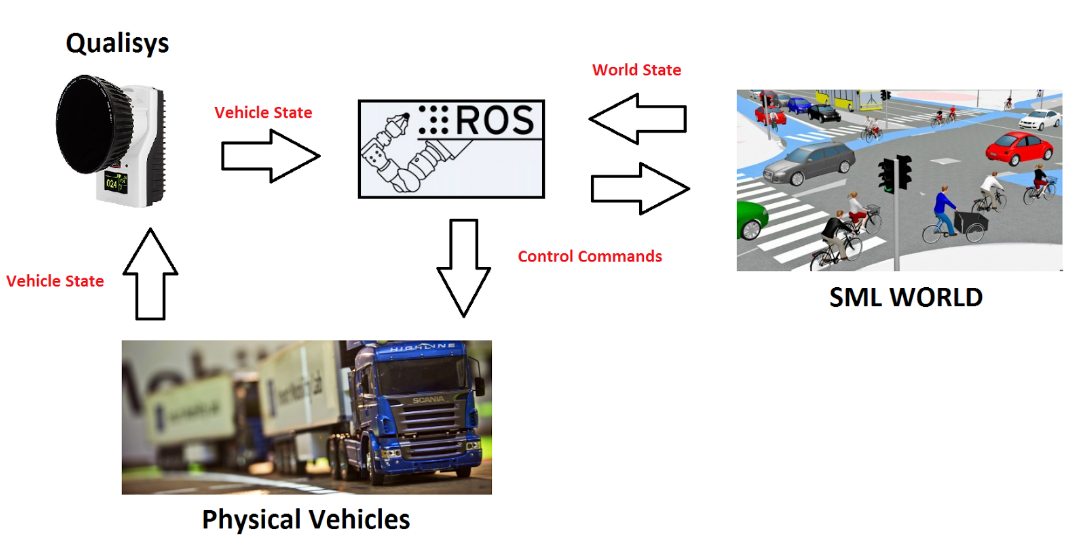
\includegraphics[width=\textwidth]{physicalvehicles.png}
  \caption{\textit{Basic communication setup between Physical and Simulated world.}}
\label{fig:setup}
\end{figure}

\subsection{Radar Integration}
The physical vehicles are equipped with Ultrasonic sensors that are controlled using an Arduino on board the truck. See Figure \ref{fig:ultrasonic}

\begin{figure}[!ht]

  \centering
    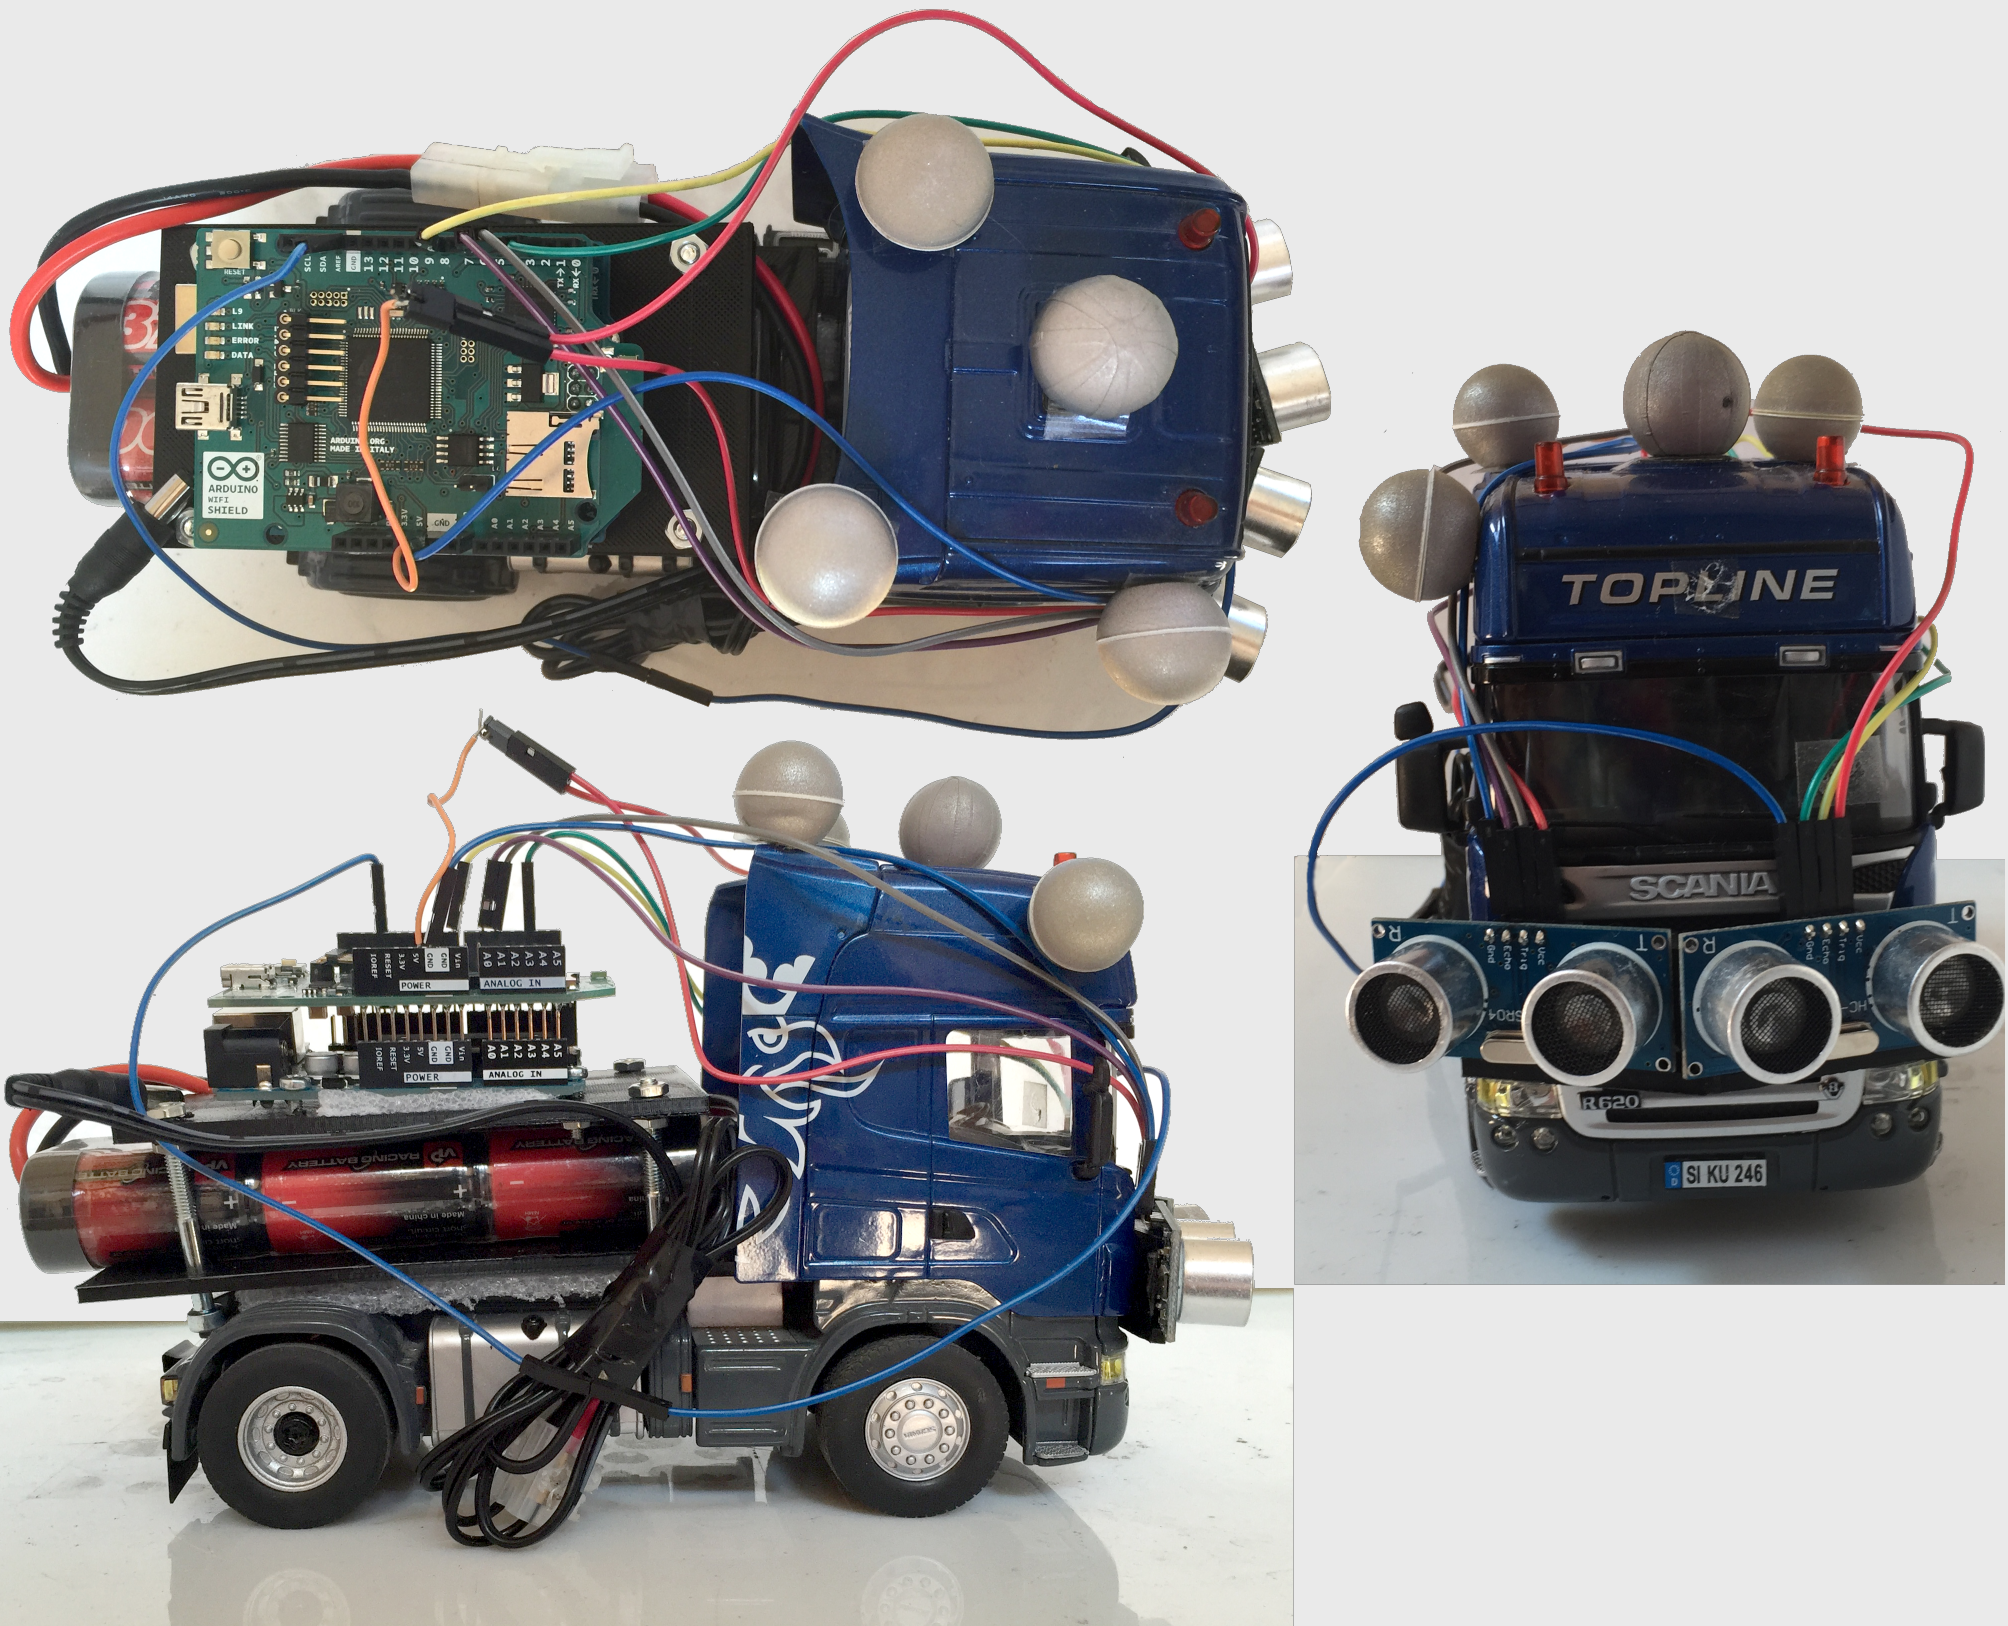
\includegraphics[width=\textwidth]{truck.png}
  \caption{\textit{1:32 Siku truck with ultrasonic sensors mounted.}}
\label{fig:ultrasonic}
\end{figure}

\subsection{Communication with SML World}
The communication between the Physical vehicles and SML world goes via Robotic Operating System (ROS) and the Motion Capture System (Qualisys). \\

\noindent The state of the physical vehicles is effectively captured by Qualisys, which is able to give up to six degrees of freedom (x, y, z, roll, pitch, yaw). This data is passed on to ROS where the high level controller computes the next set of control commands.

\subsection{List of necessary hardware}
To run the trucks in the above described setup the following devices are required and available in the SML:
\begin{itemize}
\item 1:32 Siku RC truck(s)
\item Arduino(s)
\item Arduino wifi shield (two available int the lab)
\item Wireless nano USB adapter (one Edimax 150Mbps available in the lab)
\item Ultrasonic sensors (three available in the lab)
\end{itemize}

\chapter{User Interfaces}
\section{Terminal based interface}
Generally terminals are used to run SML World demonstrations, as the terminal enables easy access to all ROS programs and commands.

\section{Graphical user interface}
Several GUIs are available for running SML World and its features. A GUI is often demonstration specific and will contain tools for the specific commands required by that demo. The following GUI:s are currently available in the SML World repository:
\begin{itemize}
\item SML Command Central (sml\_world\_start.py)
\item Intelligent traffic demo GUI (nico\_GUI.py)
\item CMA presentation GUI (CMA\_presentation\_GUI.py)
\end{itemize}

\noindent The SML Command Central allows the user to configure and run SML World with minimal use of the terminal. Note that ROS will have to be sourced and that the desired map must have a generated bpm file for this to function. \\


\part{User Manual}


\chapter{Running SML World}
\section{Preparing to run SML World}

\subsection{Required third-party software}
\begin{itemize}
\item ROS (indigo or higher)
\item python 2.7
\item git
\item pygame
\item compiz (compizconfig-settings-manager compiz-fusion-plugins-extra compiz-fusion-plugins-main compiz-plugins)
\item numpy (1.9 or higher)
\item Gtk3 (optional)
\item ELO touch screen driver (optional)
\end{itemize}

\subsection{SML source code}
\label{sec:sourcecode}
Currently the SML World source code is located in the KTH GitHub Enterprise repository https://gits-15.sys.kth.se/.
A KTH.SE account is required to be granted access. Follow instructions on the KTH website to activate the github user account connected to a specific KTH.SE acocunt. \\

\noindent The following instructions assumes the user will contribute to the project using git. Any user that will not develop nor modify any code can skip steps 4-5 in the list below.
\begin{enumerate}
\item Setup a catkin workspace for your own ROS packages (indigo or higher) according to instructions in RD2.
\item Go to the 'src' folder of your catkin workspace. 
\item Clone git repository. Note that SSH must be used for cloning (not https).
      \begin{itemize}
        \item git init
        \item git remote add origin <git-repository url>
        \item git pull origin master
      \end{itemize}
\item Set git configurations:
      \begin{itemize}
        \item git config --global user.name <username>
        \item git config --global user.email <email>
      \end{itemize}
\item Create the file '.gitignore' and add the following lines:
      \begin{itemize}
        \item .gitignore
        \item /CMakeLists.txt
        \item *.pyc
      \end{itemize}
\end{enumerate}


\subsection{Notes on SML World scenarios}
The SML World is generally modified and developed based on the specific features desired to showcase in an upcoming demonstration in the lab. This subsequently has given rise to different \textit{scenarios} in the sml\_world package. As a consequence of this, not all existing features are compatible. 

\subsection{Configure pygame}
Resizing the pygame display to fit a specific monitor or projector can be done by modifying the visualization.py script. The lines at the end of the script determines the size of the pygame window as shown below, where the values \textit{1920, 1080, 5} correspond to desired width, height and resolution (pixels per meter) and the boolean (below set to False) will crop the window if set to True.

\begin{verbatim}
vis_module = Visualization(base_path, map_location, 
                              1920, 1080, 5, False, 
                              sys.argv[1] == 'True',
                              sys.argv[2] == 'True', 
                              sys.argv[3] == 'True')
\end{verbatim}

\noindent Use compiz (listed in required third-party software above) to enable relocation of the pygame window between different monitors and projectors.

\subsection{Configure launch files}
A launch file defines a series of nodes to be started consecutively using the command line ROS program roslaunch (rosluanch <\textit{package\_name}> <\textit{launch\_file}>). A ROS service can also be called from a launch file, which should then be handled as a separate node. Some nodes might require arguments as input. The following is an example of a launch file for the SML World: \\

\begin{verbatim}
<launch>
  <node pkg="sml_world" name="road\_network" type="road_network.py" 
        args="/resources/scenarios/KistaDemo3 False False False" />
  <node pkg="sml_world" name="visualization" type="visualization.py" 
                                        args="False False False" />
  <node pkg="sml_world" name="sml_world_central" 
                                     type="sml_world_central.py" />
  <node pkg="rosservice" name="spawn_vehicle" type="rosservice" 
                               args="call --wait /spawn_vehicle 
                                    '{vehicle_id: 1, class_name: 
                                 'DummyVehicle', x: 0.0, y: 0.0, 
                               yaw: 0.0, v: 10.0, node_id: -400, 
                                             toggle_sim: true}'" />
</launch>
\end{verbatim}

\noindent The above launch file will start four nodes - three from the sml\_world package and one node corresponding to a ROS service call that will spawn a vehicle. Note that the --wait argument is necessary for letting the three sml\_world nodes start up fully before the service is called. The three sml\_world package nodes are essential for running SML World. The nodes road\_network and visualization nodes require some arguments to be set. Their arguments are defined as follows: \\
\begin{itemize}
\item Road network: <map> <traffic bool> <traffic light bool>
\item Visualization: <traffic bool> <traffic light bool> <sensor bool>
\end{itemize}

\subsection{Notes on running SML World across multiple machines}
The information in this section is merely intended as an addition to the guide \textit{Running ROS across multiple machines} available on the wiki in RD2.

\section{Running SML World}
\subsection{Using command line}
The following steps assumes that the SML World source code has been downloaded and that a catkin workspace has been set up according to instructions in section \ref{sec:sourcecode} above. The instructions below are also available on the project repository wiki under \textit{Running sml\_world for the first time}.

\begin{enumerate}
\item Set up ROS with:
	\begin{verbatim}
	source /opt/ros/indigo/setup.bash
	\end{verbatim}
\item Go to the root folder of the catkin workspace (normally 'catkin\_ws') and build the ROS package inside the 'src' folder with:
	\begin{verbatim}
	catkin_make
	\end{verbatim}
\item The successful build will create two new catalogues - 'devel' and 'build'. Finish the set up by running:
	\begin{verbatim}
	source devel/setup.bash
	\end{verbatim}
	Note that this step needs to be repeated for each new terminal.
\item Launch the key SML World ROS nodes using the launch file described above with:
	\begin{verbatim}
	roslaunch sml_world starter.launch
	\end{verbatim}
\end{enumerate}

\noindent This will launch all the key features of SMl World. The simulation can be manipulated in several ways, e.g. multiple vehicles, pedestrians and radio controlled cars can be added. Spawn additional vehicles by calling the ROS service \textit{spawn\_vehicle} in a new terminal by using the following command:

\begin{verbatim}
rosservice call /spawn_vehicle '{vehicle_id: <positive int>, 
class_name:'<class name>', x: <float>, y: <float>, yaw: <float>, 
v: <float>, node_id: <node id>, toggle_sim: <bool>}'
\end{verbatim}

\noindent By typing \textit{rosservice call /spawn\_vehicle} and then using the tab key to auto-complete a template of the necessary arguments will be generated. The arguments can be described as follows:
      \begin{itemize}
        \item 'vehicle\_id': a \textit{unique} positive integer. Note that no two vehicles can have the same ID, attempting that would result in both vehicles crashing immediately. 
        \item 'class\_name': any availbale SML World vehicle class, refer to section \ref{sec:vehicles} above. 
        \item 'x', 'y' and 'yaw': any point on the pygame window where the vehicle is desired to first appear. The origin is defined in the XML file that makes up the road network and the yaw is measure from the horisontal axis of the pygame window. 
        \item 'v': a positive float corresponding to speed in meters per second, normally 0>v>20. 
        \item 'node\_id': will determine the trajectory of the vehicle (that can later be changed) as described in section \ref{sec:road} above. 
      \end{itemize}

\noindent Examples of arguments:

\begin{verbatim}
rosservice call /spawn_vehicle '{vehicle_id: 3, class_name:
'DummyVehicle', x: 0.0, y: 0.0, yaw: 0.8, v: 15.0, node_id: 
-400, toggle_sim: true}'
\end{verbatim}

\subsection{Using the GUI}

\begin{figure}[!ht]

  \centering
    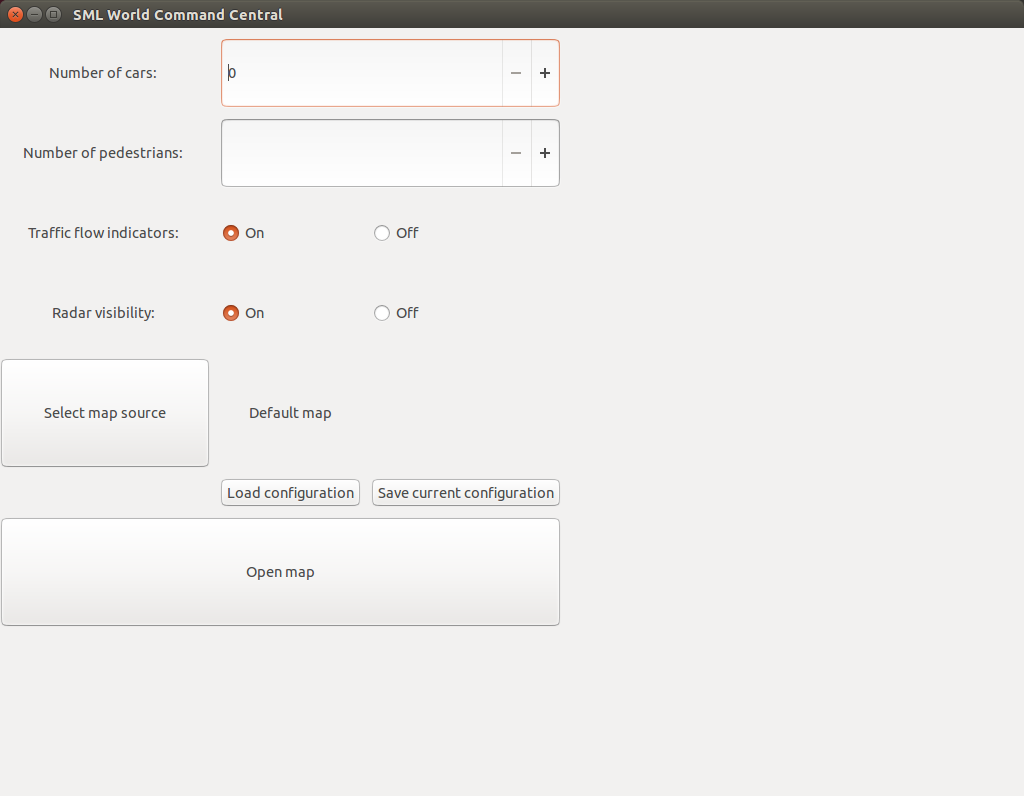
\includegraphics[width=0.8\textwidth]{smlcommandcentral.png}
  \caption{\textit{The SML Command Central that allows configuring and running SML World.}}
\end{figure}

\noindent The latest version of the GUI developed to be used with the ELO touch screen is \textit{sml\_world\_start.py} located in sml\_world/scripts/user\_interfaces. This is also compatible with any regular PC monitor. It will allow the user to select the desired number of cars, whether to activate traffic lights, traffic flow analysis, radar visualzation and generate pedestrians and crosswalks. It also lets the user select a map from the existing set of XML-based bpm files. Note that if the bpm has not been generated this feature will not work properaly as the GUI cannot generate it separately. In such a case it is most conventient to run roslaunch with the desired configuration once. The GUI also allows the user to save the current configuration that has been put together in the GUI and/or to load a previously stored configuration. A configuration is automatically named \textit{customstarter + <current date><current time>.launch} when saved. Clicking \textit{Open map} will start SML World with the selected configuration. 


\section{Start radio controlled trucks}
Start vehicle simulation using class \textit{TruckVehicle}.

\begin{figure}[!ht]

  \centering
    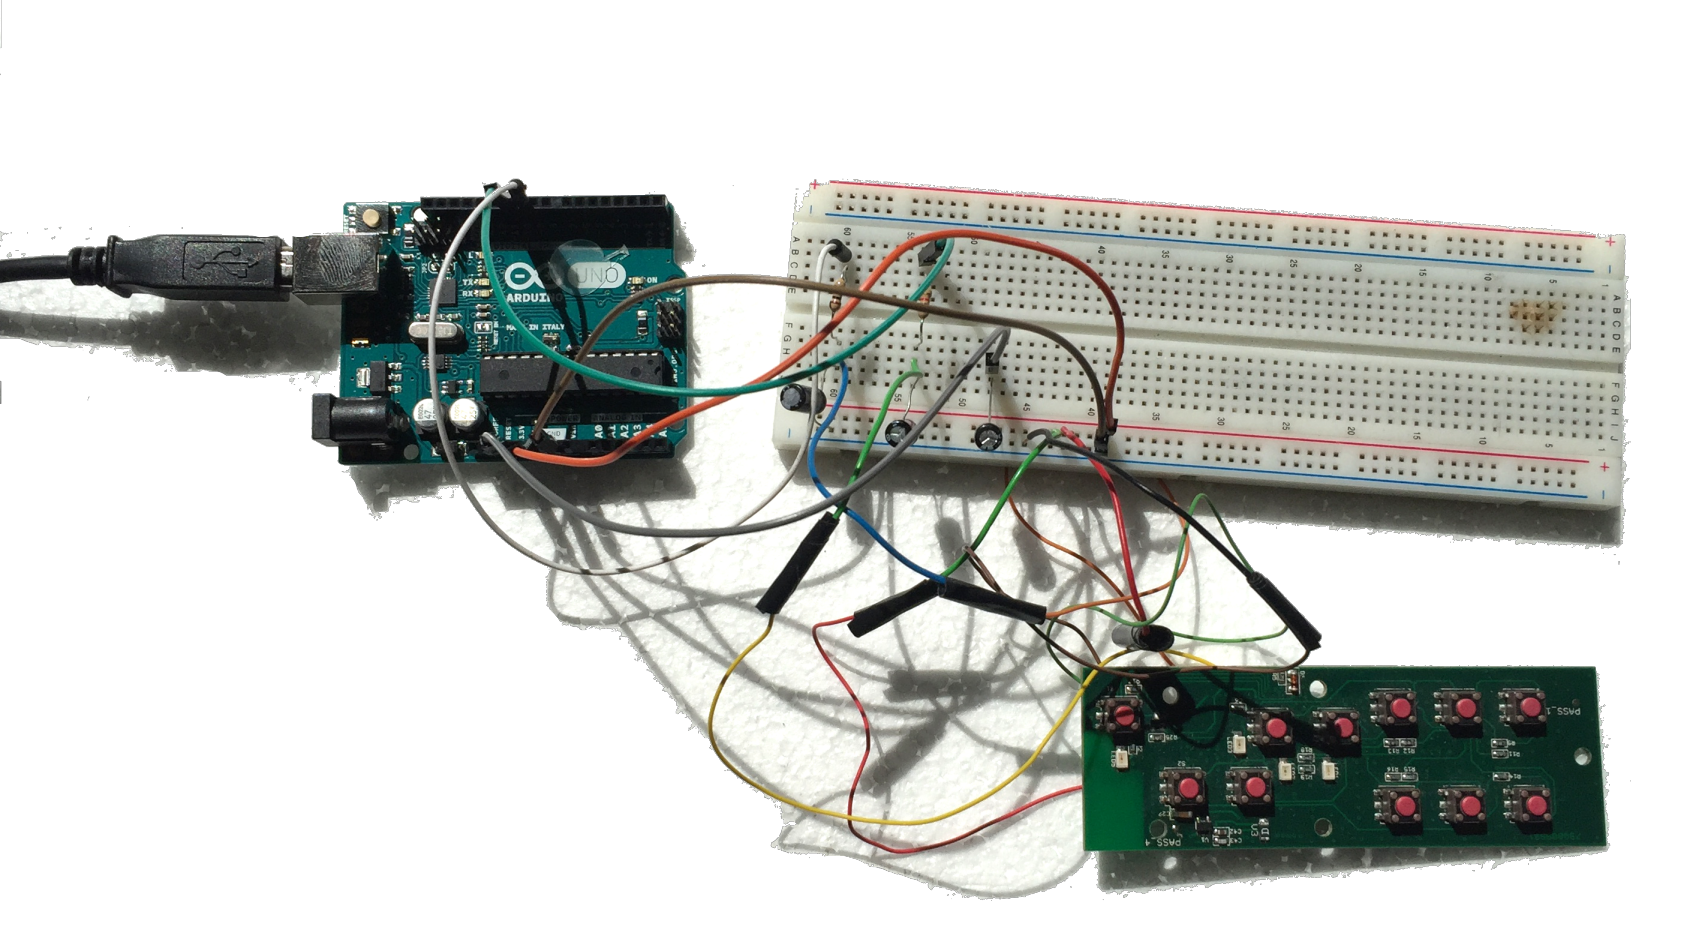
\includegraphics[width=\textwidth]{breadboard.png}
  \caption{\textit{Bread board connections. USB cable connected to the PC, which in turn has an Edimax USB wifi module. Components: Arduino Uni, remote control of the truck}}
\end{figure}

\subsection{Shutdown}
The current version can be killed using the escape key.

\end{document}
